\providecommand{\muh}{\hat{\mu}}
\providecommand{\yh}{\hat{y}}

\chapter{\label{chap:intro} Introduction}

% Motivation.1: information summarization.
One of the most exciting challenges in natural language processing is the development of applications that can summarize information for us.
For example, text summarization systems (\reffig{intro:overview-summarization}) seek to identify the most salient information contained within one or more related articles and synthesize this information in as few words as necessary.
Knowledge base population systems (\reffig{intro:overview-kbp}) read documents from a large corpus or the Internet and present succinct, structured, summaries about the people and organizations mentioned within.
Finally, at the other end of the spectrum, open-response question answering systems (\reffig{intro:overview-qa}) provide exactly the information required to answer a particular question.

\begin{figure}
  \centering
  \begin{subfigure}{0.45\textwidth}
    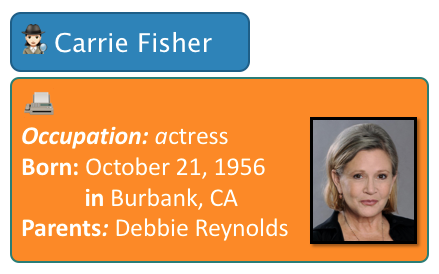
\includegraphics[width=\textwidth]{figures/overview-kbp}
    \caption{\label{fig:intro:overview-kbp} Knowledge base population.}
  \end{subfigure} \\
  \begin{subfigure}{0.55\textwidth}%
    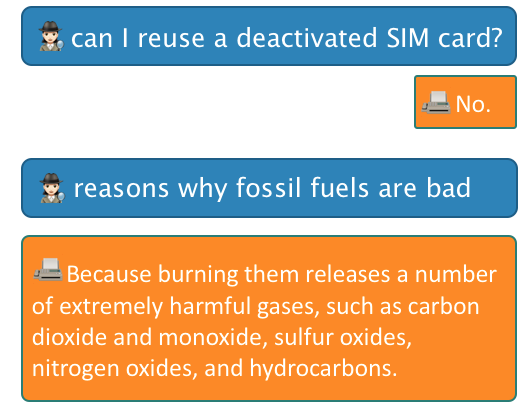
\includegraphics[width=\textwidth]{figures/overview-qa}
    \caption{\label{fig:intro:overview-qa} Open-response question answering.}
  \end{subfigure} \\
  \begin{subfigure}{0.55\textwidth}
    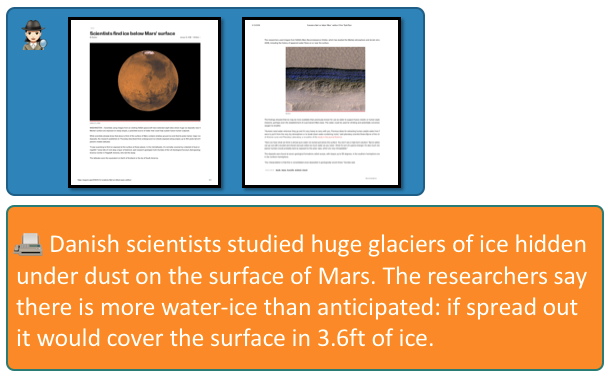
\includegraphics[width=\textwidth]{figures/overview-summarization}
    \caption{\label{fig:intro:overview-summarization} Text summarization. }
  \end{subfigure}

  \caption{\label{fig:intro:overview} An overview of some information summarization tasks.
  (a) Knowledge base population: reads documents from a large corpus and generates linked entity-centric summaries for every person and organization mentioned within.
  (b) Open-response question answering: provides very-targeted summaries that address a specific question.}
  (c) Text summarization: seeks to identify the most salient information contained within one (or more) article(s) and describe this information in as few words as necessary.
\end{figure}

% Motivation.2: Status quo is broken. 
Despite a long history of work on these problems, current systems still fall short of their promise (see \reffig{intro:example-fails} for some \ac{examples}).
There are many reasons for this gap in performance, but we believe that one key reason is the lack of an effective evaluation methodology.
At its core, the current evaluation methodology was developed with classification problems in mind where each output belongs to a (typically small) closed class, e.g.\ positive and negative sentiment.
As a result, given a reference answer it is very easy to determine whether or not a classification system's output is correct or not.
The classification paradigm of evaluation then is to simply collect an evaluation dataset with a large number of input-output pairs and to measure how many of these pairs a system is able to correctly predict.

Unfortunately, for tasks we are interested in, it is either impossible to collect this test set or there exist many genuinely correct responses for a single input.
Either way, our evaluation data is fundamentally \textit{incomplete} and is unable to judge the output produced by systems.

\begin{figure}
  \centering
  \begin{subfigure}{0.65\textwidth}
    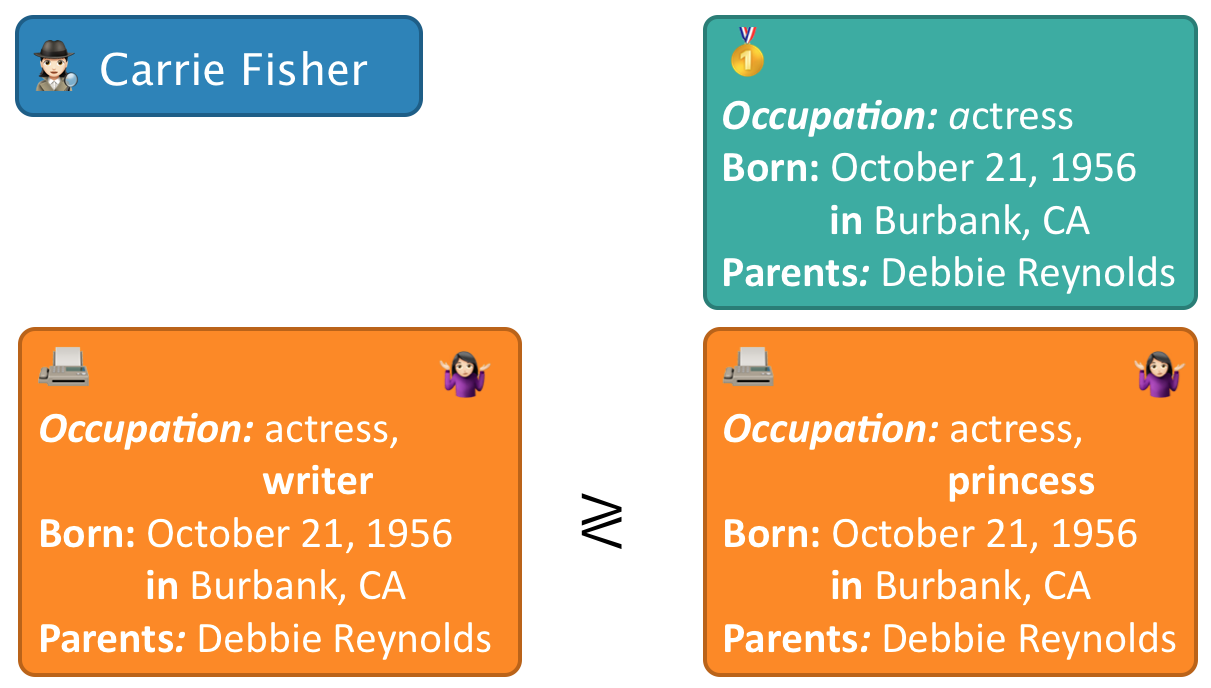
\includegraphics[width=\textwidth]{figures/example-kbp}
    \caption{\label{fig:intro:example-kbp} Knowledge base population.}
  \end{subfigure} \\
  \begin{subfigure}{0.65\textwidth}%
    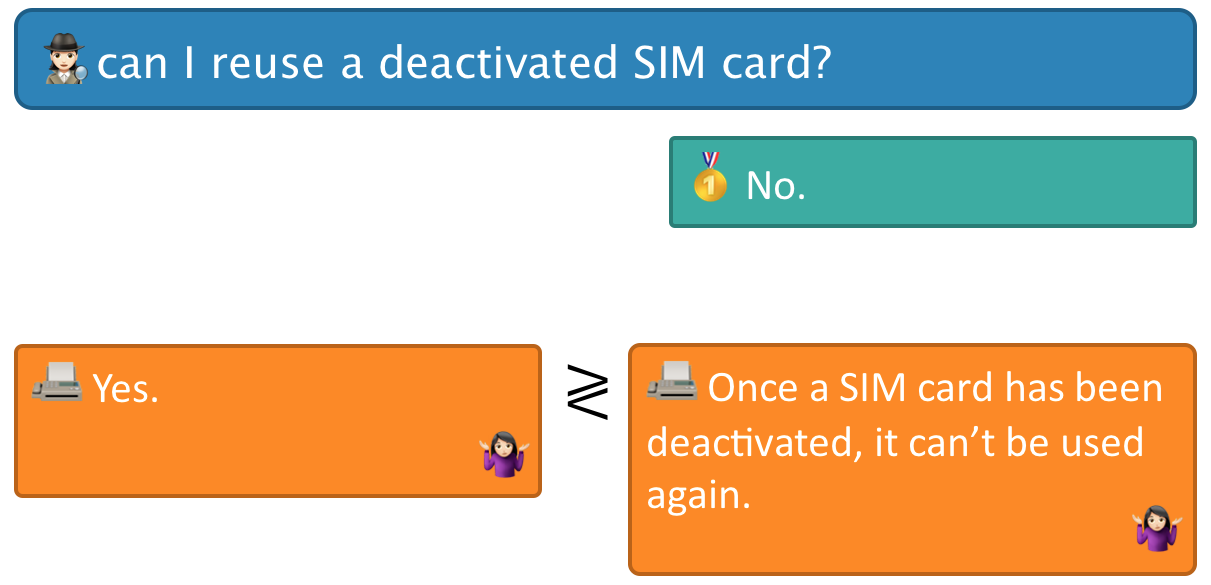
\includegraphics[width=\textwidth]{figures/example-qa}
    \caption{\label{fig:intro:example-qa} Open-response question answering.}
  \end{subfigure} \\
  \begin{subfigure}{0.65\textwidth}
    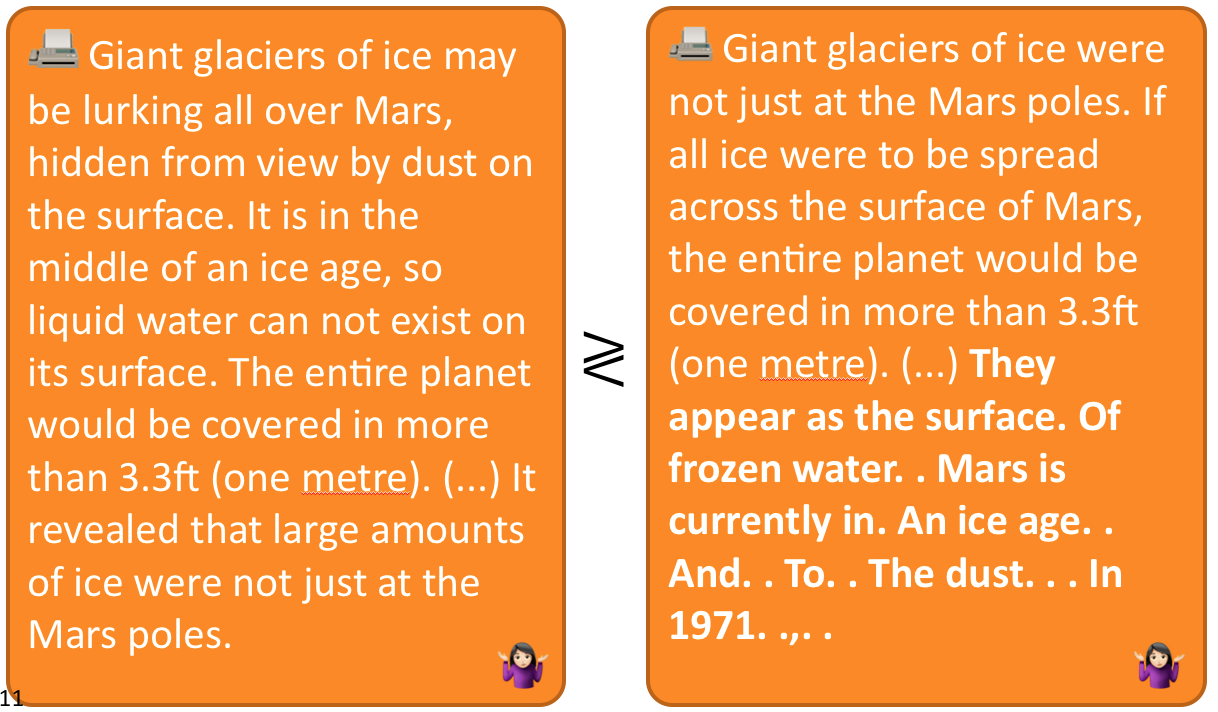
\includegraphics[width=\textwidth]{figures/example-summarization}
    \caption{\label{fig:intro:example-summarization} Text summarization. }
  \end{subfigure}
  \caption{\label{fig:intro:examples} Examples where the reference   data is unable to evaluate a system's response:
  (a) Knowledge base population: here, the incomplete reference data is unable to identify that it is a true that Carrie Fisher was also an author, but not that she is a `princess'.
  (b) Open-response question answering: it is common for systems to output a paraphrase of the reference answer and thus to be judged incorrect despite reporting the right answer.
  (c) Text summarization: systems rarely produce output that is identical to the reference answer and word-overlap based similarity measures often prefer bad responses with high lexical similarity over good responses that more more lexically distinct.  
  }
\end{figure}

Let's look at some examples of how this manifests in practice:
\reffig{intro:example-kbp} shows the candidate output of two KBP systems for Carrie Fisher, the late actress who played Princess Leia in the Star Wars movie franchise.
The incomplete KBP reference data only specifies that Carrie is an actress and thus the evaluation is unable to judge whether the system that identifies her to also be an author (which is correct) is better or worse than one that identifies her to also be a princess (which is incorrect).
Next, consider an example in question answering: there are many ways to express the same answer as shown in \reffig{intro:example-qa}. Unfortunately, our evaluation dataset contains only one of them, and the system is marked incorrect.
Finally, consider the evaluation of summarization: a system generated summary will never exactly match the one in the gold dataset.
A common practice in the community is to use a word-overlap based similarity score such as BLEU or ROUGE\@.
This has its dangers as there are many bad summaries that have a high word overlap, and many good summaries that do not. \reffig{intro:example-summarization} shows an example of a system that generated a summary to score high on this metric by appending seemingly random words at the end.

A common theme across all these examples is that we have an ``incomplete'' evaluation dataset that makes it hard to compare two systems.
Naively using the dataset may lead to statistically invalid conclusions.
Even worse, we will show that many accepted methods to construct evaluation datasets are biased towards certain types of systems and thus negatively penalize valuable research directions that do not conform to the implicit assumptions of the evaluation.
For example, in knowledge base population, we show that the current evaluation is heavily biased against novel systems that identify true facts (e.g. Carrie Fisher being an author) that no other system has.
In summarization, the evaluation is biased towards systems that are lexically similar to the reference summary even if it is grammatically nonsensical.
\citet{connor2010mind} show that similar bias towards lexical similarity led over time to the development of systems that do better at the ROUGE metric without significantly improving on human evaluation.
Just as a sturdy ladder makes it easy to climb higher, a good evaluation methodology would allow us to improve our systems one small step at a time.

As a consequence of these observations, the only reliable way to evaluate systems for these tasks at present is to do a human evaluation.
Unfortunately, human evaluation can be quite expensive and impractical.

The key question this thesis tries to answer then is: ``can we reliably reduce the cost of human annotation in evaluation''?
We find that we can classify problems in two categories based on how often two different systems may produce the same output (\reffig{dense-sparse}).
When it is likely that two systems produce an overlapping set of output (``dense''), we may can leverage any human annotations we obtain on one system on another.
The key challenge then is how to guard against a representation bias: if all the systems predict in an ``easy'' region, we may expect the evaluation to be tilted in favor of easy examples and lose its ability to discriminate between systems.
We tackle this problem by using a novel importance-reweighted estimator in \refchap{kbpo} and show how it can be applied to evaluate knowledge base population systems to reduce the cost of obtaining human annotations by a factor of 4.

On the other end of the spectrum, in tasks like text summarization, it is extremely unlikely that two systems exactly agree on any output they produce.
Here, it seems natural to rely on some ``similarity'' measure that may allow us to match two similar, but non-identical responses.
Indeed, this is the role of automatic metrics such as BLEU or ROUGE.
Unfortunately, automatic metrics have been reported to have poor correlations with human judgment and thus 
In \refchap{price}, we look at bias introduced through such metrics and ...

Equally important to comparing systems is understanding their failings in order to improve them.
How we can use human feedback here.

Find limitations of unbiasedness.

Thus far, we have focused on the use of human feedback during evaluation.
In \refchap{otj}, we show how human feedback can be effectively integrated \textit{a test-time}.
We consider an ``on-the-job'' setting, where as inputs arrive, we use real-time crowdsourcing to resolve uncertainty where needed and output our prediction when confident.
As the model improves over time, the reliance on crowdsourcing queries
decreases. 
We cast our setting as a stochastic game based on Bayesian decision
theory, which allows us to balance latency, cost, and accuracy objectives in a principled way. 
Computing the optimal policy is intractable, so we develop an approximation based on Monte Carlo Tree Search.
We tested our approach on three datasets---named-entity recognition, sentiment classification, and image classification.
On the NER task we obtained more than an order of magnitude reduction in cost compared to full human annotation, while boosting performance relative to the expert provided labels.
We also achieve a $8\%$ \fone{} improvement over having a single human label the whole set, and a $28\%$ \fone{} improvement over online learning.


% In other situations, such as performing information extraction on the web, the collection of inputs that express a particular concept may itself be so varied that it is unrealistic to expect that we may cover them in a static training dataset.
% Finally, in the context of automatic text generation, the assumption that there exists a single well-defined ``correct'' output is broken.
% 
% % What happens when the data we need for learning systems is not collectible?
% 
% % We explore using human feedback in these settings.
% 




% In natural language tasks such as knowledge base population, text summarization or open-response question answering, a significant challenge is simply evaluating the performance of automated systems because of the large diversity of possible outputs.
% % ^^ Include the fact that the domain has shifted?
% Existing fully-automatic methods for evaluating these systems rely on an incomplete set of annotated references which lead to systematic biases against certain system improvements: in other words, genuinely good ideas are systematically discarded simply because of limitations in our evaluation methodology.
% As a result, human evaluation, which can be prohibitively expensive, has remained the de-facto mode of evaluation for these tasks.
% In this work, we show how one can decrease the costs of incorporating human feedback through the design of appropriate statistical estimators. 
% 
% First, we consider the setting where the output produced by systems is ``dense'', in that we expect significant overlap between the output of different systems. 
% Naively combining annotations from different systems leads to a representation bias.
% Here, we show that cost of obtaining human feedback can be significantly amortized by using a novel importance-reweighted estimator.  
% We apply this estimator to design a new evaluation methodology for knowledge base population and show that cost of evaluating precision and recall within this framework can be reduced by a factor of 4.
% 
% Next, we consider the ``sparse'' setting wherein few, if any, systems ever produce identical output.
% Traditionally, the community has relied on similarity-based automatic metrics such as BLEU or ROUGE to compare the outputs produced by different systems.
% Unfortunately, these metrics have been shown to poorly correlate with human judgment and thus introduce bias in evaluation.
% We derive an unbiased estimator that optimally combines these automatic metrics with human feedback.
% Our theoretical results allow us to characterize potential cost reductions only in terms of the tasks' subjectivity, measured by inter-annotator variance, and the automatic metrics' quality, measured by correlation with human judgments.
% On two popular natural language generation tasks, question answering and summarization, we empirically show that currently we can achieve at most a 7--13\% reduction in cost on two tasks, exposing fundamental limitations in debiasing current automatic metrics.
% 
% Finally, we show how human feedback can be incorporated into systems in real-time to deploy high-accuracy systems starting with zero training examples.
% We build systems that learn ``on-the-job'' by using human feedback to resolve uncertainty until it is confident in its predictions.
% Our key statistical idea here is to cast the problem as a stochastic game based on Bayesian decision theory, which allows us to balance latency, cost, and accuracy objectives in a principled way.
% When tested on three classification tasks---named-entity recognition, sentiment classification, and image classification--- we obtained an order of magnitude reduction in cost compared to full human annotation, while also boosting performance relative to the expert provided labels.
% 

% 
% 
% % We are used to supervised data specifying tasks, but this is a limiting perspective.
% One of the key insights of modern machine learning is that data provides a specification for otherwise fuzzy concepts like ``What is the sentiment expressed by this sentence?'', ``Is this sentence an example of hate-speech?'' or ``What semantic role does this word play in the sentence?''.
% Given a sufficiently large dataset of inputs paired with class labels, we have found models that are expressive enough to learn good definitions for these concepts.
% % TODO: Examples?
% % Sentiment (and other text) classification
% % Semantic role labeling and dependency parsing
% 
% Of course, there are many applications where this perspective of learning is insufficient.
% In many situations, one wishes to build a new system --- e.g., to do Twitter information extraction
% \citep{li2012twiner} to aid in disaster relief efforts or monitor public
% opinion --- but one does not have the luxury of time or resources to collect a ``sufficiently large'' dataset before deploying the system.
% In other situations, such as performing information extraction on the web, the collection of inputs that express a particular concept may itself be so varied that it is unrealistic to expect that we may cover them in a static training dataset.
% Finally, in the context of automatic text generation, the assumption that there exists a single well-defined ``correct'' output is broken.
% 
% % What happens when the data we need for learning systems is not collectible?
% 
% % We explore using human feedback in these settings.
% 
% % 1. What are the metaphors: vision of the future -- enabling applications -- needing to climb the ladder -- human feedback is the ladder -- how do we make it cheaper?
% % how do we effectively use 
% What tools must exist in the future in order to make effective use of the ever-expanding corpus of information available at our fingertips?
% Given that the working set memory of the average human being is only <>,
%   it is natural to expect that tools that 
% Here, information retrieval has already helped, but not enough.
% 
% Consider, for example, tools that allow us to summarize entire document troves to learn key information about the people mentioned within, tools that allow us to ask questions that synthesize information across these entire collections, and tools that can summarize articles.
% All of these applications have been actively pursued by the NLP community for many years and remain incredibly challenging.
% 
% No doubt, this is because of many many reasons, but one that we wish to explore here is the lack of a reliable evaluation methodology.
% Evaluation is the key ingredient that establishes a science and engineering.
% By establishing a ladder, we allow ourselves to climb up one step at a time to soaring heights.
% 
% In this metaphor, existing evaluation methodologies are broken ladders -- one step up indeed leads us two steps down.
% 
% 
% 
% Our goal is simple: to enable the development of systems that can effectively summarize information for us.
% 
% 
% 
% 
% Let us peer into a vision of the future for natural language processing:
%   all of the world's information is made available to us and we are able to ask systems 
% 
% % Where is it most cost-effective?
% 
% % Story 
% % 1. Picture of the future. Systems that can do X, Y, Z. 
% Let us 
% 
% % 2. Where we are now.
% % 3. What is holding us back?
% 
% 
% % 1. Field setup
% 
% For a long time, the natural language processing (NLP) community has striven to build a foundation to process language at the lexical, syntactic and semantic level.
% We have seen tremendous progress at identifying such low-level information as parts-of-speech and syntactic parses: today's systems certainly rival human performance on these tasks.
% 
% At the same time, we continue to struggle to understand basic semantics: transferring labels across domains,
% 
% We believe that a key challenge to solving these tasks is the absence of a ladder that will allow us to climb. 
% Hard to bootstrap -- here is where humans should come in.
% 
% Closing the loop: increase interaction, having machines synthesize responses for people.
% 
% [synthesis evaluation] --- [adaptation (also in tandem)]
% 
% what are the classification problems?
% - sentiment classification
% - abuse classification
% - intent classification
% - 
% 
%   We
% A common pattern for most of these problems is that they are classification problems.
% 
% By no means have all the key problems of natural LP -- the challenges of deep text understanding truly remain.
% As we solve these problems, 
% 
% 
% 
% In some sense, we have followed a Turin model of artificial intelligence: we set up tests and compare ourselves with a human == can we do as well as a person?
% In the world of generation this is b no means as easy to define.
% Indeed the past is littered with attempts and waves of progress.
% 
% What new tool do we have for this now?
% Crowdsourcing is thy name.
% 
% 
% The field of natural language processing has advanced to the degre
% 
% How do systems co-evolve with humans?
% People get to train on the job to learn what to do.
% We can enable this for machines too with OTJ.
% 
% % Over the last X years, we've basically solved classification.
% % The new frontier is generation, with new interest in many different tasks.
% 
% % 2. The problem: evaluation
% % A dogged problem for this field is evaluation.
% % Evaluation has been studied extensively for a long time.
% % Some of the limitations.
% 
% % 3. The enabler: crowdsourcing
% % Recent past, crowdsourcing has really enabled us to change the way we collect data and annotations.
% % At no earlier point could we interactively collect annotations.
% % But expensive.
% 
% % 4. The solution: statistical estimation.
% % Revisit evaluation, we find that there are problems with cost
% % Different settings require different solutions.
% % Sparse vs Dense.
% 
% % 5. More problems: on-the-job.
% 
% Placeholder.
% 
